\section{Templates}




\subsection{Boat}
The boat template as the name infers is a model of the real boat. 
The boat is capable of carrying at most two persons and most have at least one adult to handle the boat. 
From the initial state, called still, the only possible edge is to the one person location. 
In this edge the boat listens for a handshake on the adultOn channel. 
When a person responds to the handskake the persons sailing time is transmitted through the global variable temp_sailtime. 
A function set_sailtime is used to set the sailtime to the lowest value, so the fastest person on the boats sailing time is the one used. 
temp_sailtime is reset to reduce the state space.
7 From the One person location there are three edges. 
Two edges to the two person loaction where eihter a child or an adult embarks. 
The adultOn edge is similar to the first edge described. 
The childOn edge does not need to synchronize a sailtime since the children does not control the boat. 
From both two person and the one person location an edge to the sailing locatoin is possible. 
Here a card calls the function verify, which is described in \ref{}. 
The sailing location has an invariant that makes sure it stays in the location for atleast the time it takes for the person to sail across. 
The only possible edge from the sailing location is to arrieved. 
This edge has a gaurd to make sure that the boat arrieves when it has stayed in sailing in a period equivalent to the sail_time. 
The edge broadcasts on allDisembark and makes all persons on the boat disembark. 
The local variable boatL is fliped to note that the boat has changed site. 
After the disembarkment the sail time is reset to the maximum sailtime and the postion of the people is verifyed. 
\begin{figure}%
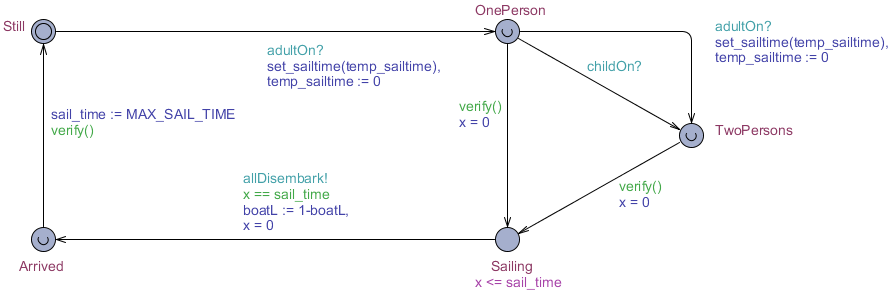
\includegraphics[width=\columnwidth]{pictures/boat.png}%
\caption{}%
\label{}%
\end{figure}
















\subsection{Person}
The person model encapsulate a single person.
When instantiated it takes three arguments.
These arguments determines which type of person is being instantiated and how it should interact with the rest of the system.
The arguments that a person needs to be instantiated are: A channel, a person type, and a sail time.
The channel argument is used to signal that the given instance gets on the boat.
The person type indicates what kind of person is being instantiated, e.g. a boy.
The sail time is only applicable to the mom, dad, and police officer.
It is part of the 2nd task, which is to add temporal constraints and have each of the adults cross the river with different speeds.
\begin{figure}%
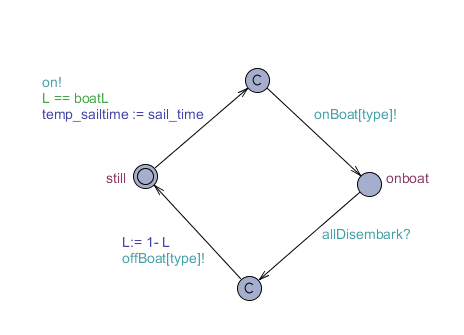
\includegraphics[width=\columnwidth]{pictures/person.png}%
\caption{The timed automata for a person}%
\label{fig:person}%
\end{figure}

The timed automata of a person seen in Figure \ref{fig:person} shows four circular connected locations.
The two locations OnBoat and OnLand indicate the current position of the person.
These names should be self-explanatory.
The local variable L is used to indicate which side of the river the person is on.
0 is left and 1 is right.
This variable is used to check that a person instance can only embark when it is on the same side as the boat.
L is update when a person as crossed the river and enters the location OnLand again.

The locations ToBoat and ToLand are intermediate states.
These are needed because there is a handshake with the boat and a broadcast to the observer whenever a person embarks or disembarks.
When a person embarks the reader can think of it as the person first jumps on the boat (taking the edge from OnLand to ToBoat) and immediately afterward reports to the observer (taking the edge from ToBoat to OnBoat).
Similarly when a person instance disembark it starts out by leaving the boat (or rather being forced to leave, since it is the boat that does the output on the allDisembark channel) and then reports to the observer.
















\section{Observer}
\begin{figure}%
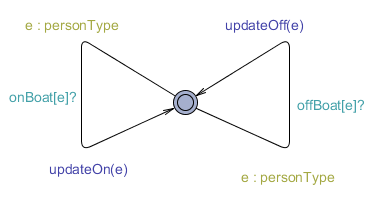
\includegraphics[width=\columnwidth]{pictures/observer.png}%
\caption{}%
\label{}%
\end{figure}




























\section{Observer}